\documentclass[10pt,twocolumn,letterpaper]{article}

\usepackage{cvpr}
\usepackage{times}
\usepackage{epsfig}
\usepackage{graphicx}
\usepackage{amsmath}
\usepackage{amssymb}


% Include other packages here, before hyperref.

% If you comment hyperref and then uncomment it, you should delete
% egpaper.aux before re-running latex.  (Or just hit 'q' on the first latex
% run, let it finish, and you should be clear).
\usepackage[pagebackref=true,breaklinks=true,letterpaper=true,colorlinks,bookmarks=false]{hyperref}

\hypersetup{
    colorlinks=true,
    linkcolor=blue,
    filecolor=blue,      
    urlcolor=blue,
}

% \cvprfinalcopy % *** Uncomment this line for the final submission

\def\cvprPaperID{****} % *** Enter the CVPR Paper ID here
\def\httilde{\mbox{\tt\raisebox{-.5ex}{\symbol{126}}}}

% Pages are numbered in submission mode, and unnumbered in camera-ready
\ifcvprfinal\pagestyle{empty}\fi

\begin{document}

%%%%%%%%% TITLE
\title{Deep Cooperative Neural Network (DeepCoNN) for Movie Rating Prediction}

\author{Colby Wise\\
Columbia University\\
{\tt\small cjw2165@columbia.edu}
\and
Michael Alvarino\\
Columbia University\\
{\tt\small maa2282@columbia.edu}
\and
Richard Dewey\\
Columbia University\\
{\tt\small rld2126@columbia.edu}
}

\maketitle
%\thispagestyle{empty}

%%%%%%%%% ABSTRACT
\begin{abstract}
For our project we implemented the Deep Cooperative Neural Network (DeepCoNN) architecture outlined in the arXiv working paper "Joint Deep Modeling of Users and Items Using Reviews for Recommendation" (Zheng, Noroozi, et. al. 2017) to predict user movie ratings from user review text data. The DeepCoNN methodology models users and items jointly using review text in two cooperative neural networks. One network learns feature representations from groupings of users and their reviews, while the other network learns features from items and user reviews; both networks share a final interaction layer. This paper describes our implementation of DeepCoNN architecture using movie review data and presents results and extensions to the DeepCoNN model.
\end{abstract}
\ \newline
\href{https://github.com/michaelAlvarino/Deep-Learning}{Project GitHub Repository}

%%%%%%%%% BODY TEXT
\section{Introduction}

\par The literature on recommendation systems is deep and until recently has traditionally focused on well-known matrix factorization algorithms, such as collaborative filtering ($CF$), as popularized by Netflix and Spotify. Collaborative filtering is advantageous to other methods because it is relatively easy to implement and computationally efficient. On the other hand, the drawbacks of collaborative filtering in real-world applications lead to at times insurmountable challenges. To clarify, CF suffers from the "cold-start" problem in that it requires user ratings to make predictions. When users have no or limited prior ratings history relative to the total amount of items to rate this is called data \textit{sparsity}. For sparse user data it's difficult to accurately predict ratings/recommendations thus leading to poor model performance and generalization [9]. 

\par Recently strong empirical results in Deep Learning particularly in natural language modeling via convolutional neural networks ($CNN$) and recurrent networks ($RNN$) to capture complex feature interactions in textual data have lead recent recommendation systems ($RecSys$) research to leverage  deep learning. CNN models [1] and RNNs [3], such as \textit{Long Short-Term Memory} (LSTM) and \textit{Gated Recurrent Units} (GRU) have shown the ability to help with the generalization problem and improve model accuracy in textual data sets.

\subsection{Related Work}
Our experiments focus on expanding the $DeepCoNN$ model thus our primary reference will be the original \textit{Joint Deep Modeling of Users and Items Using Reviews for Recommendation} paper. While the authors do not provide an open-source code repository on-line, after reaching out them via email they provided guidance on model replication. Additionally, we found a similar code base on-line that utilized video game review data [8]. Related papers we referenced for re-constructing $DeepCoNN$ are $DeepFM$ [4] which similar to our model, combines a form of matrix factorization to capture user/item interactions with a CNN architecture; $TransNets$ [3], which extends $DeepCoNN$ to examples where the users review is not available. For background on factorization machines we referenced \textit{Factorization Machines} [2]. 


It should be noted that our original proposal was to replicate Google's \textit{Wide \& Deep} model [5]. We spent a considerable amount of time going down this path, but ultimately came to the conclusion that we could not source similar high quality categorical data as per the original paper. Furthermore, we decided to switch to the $DeepConn$ model due to it's greater relevancy to our data set and given the success of the paper which was recently accepted into the 2017 ACM International Conference on Web Search and Data Mining ($WSDM$). Lastly, we found the paper to be more innovative and challenging.

%-------------------------------------------------------------------------
\section{Methodology}
This section outlines the methodology used in the project including an overview of the problem formulation, an overview of our data set and preprocessing, and details of model architectures.

\subsection{Problem Formulation}

\textit{In order to make better movie recommendations how can we more accurately predict a users rating for an unseen movie based on what the user has previously seen? Furthermore, can we improve generalization of our model when information on a users past movie ratings is limited by utilizing user review data?}\\

These two questions are the crux of our problem. Prior to deep learning, standard approaches for recommendation systems ($RecSys$) used collaborative filtering which relies on decomposing users, items (i.e. movies), and ratings into latent feature matrices. The interaction between users and items is captured by matrix multiplication of the weight matrices of these latent features. One common CF method includes using the cosine similarity measure between all pairs of movies that users have rated:\\

Where,
$m_{i}$ and $m_{j}$ refer to movie vectors of ratings of users who have rated both movies:

\begin{center}
\textbf{$cos(\theta)$} =
$\frac{\vec{m_{i}} \bullet \vec{m_{j}}}{||\vec{m_{i}}||_2 \times ||\vec{m_{j}}||_2}$
\end{center}

This yields a movie-to-movie similarity matrix of dimensions $M \times M$ with ones along the diagonal. Thus, the predicted rating for movie $m_{2}$ for $user_1$ would be calculated using similarity measures between ($m_2,m_1$) and ($m_2,m_3$) weighted by the respective ratings for $m_1$ and $m_3$. 

From the above formulation we can clearly see the major disadvantage of this approach: $sparsity$. When ratings are limited the movie-to-movie matrix is mainly zeros thus limiting predictive ability. Current research like $DeepCoNN$ have attempted to improve accuracy of sparse data by using text data that users write after watching movies. This text data is used as input for training neural networks and offers additional insights versus only numerical ratings.

\subsection{Data Overview \& Preprocessing}
The Amazon Instant Video Review 5-core data is a JSON file with nine values per entry of which we use the following four:\\
\ \newline
 \hspace*{10mm}  \textbf{ReviewerID} - \textit{user ID} \\ 
 \hspace*{10mm}  \textbf{Asin} - \textit{movie ID} \\
 \hspace*{10mm}  \textbf{ReviewText} - \textit{review text} \\
 \hspace*{10mm}  \textbf{Overall} - \textit{movie rating} 

\subsubsection{Grouping Users \& Reviews}
The DeepCoNN model formulation that we'll focus on in this research uses two jointly modeled neural networks. The first network $Net_{i}$ uses all of the text reviews for a given user. The second network $Net_{p}$ uses all of the text reviews for a particular item (movie). To replicate the paper, we group users with all their reviews and movies with their reviews into two dictionaries such that each key in the dictionary is a unique $reviewerID$ ($Asin$) accompanied by a list of text reviews. 

\subsubsection{Data Preprocessing}
\begin{figure}[!ht]
\begin{center}
{\small
\begin{tabular}{l|ccccccc}
\hline
%Category & Experiment Summary  \\ \hline
 & \# Reviews & \# Users & \# Movies & Training\% & Test\% \\
\hline
Data & 18,563  & 5033 & 1685 & 90\% & 10\%  \\
\hline
\end{tabular}
}
\end{center}
\caption{Amazon Instant Video Dataset Overview}
\end{figure}

Using Keras built-in preprocessing API each review is tokenized into separate lowercased words with all punctuation removed. Then we use our embedding mapper to transform all reviews into their GloVe vector representation. Given review lengths typically differ in the number of words per review, prior to aggregating all user reviews and movie reviews into input matrices we pad ($truncate$) reviews such that input matrices are of equal dimensionality. It's important to note that our original data set includes 37,000 ratings however of these there are only 18,563 text reviews. Given we are training our model on text reviews, we limit our data set to only ratings that have reviews, thus truncating our data set down to 18,563 from 37,000. The 18,633 unique reviews are comprised from 5033 unique users and 1685 respectively. Hence on average there are 3.70 reviews/user and 11 reviews/movie. Lastly we split this data set into a randomized training and test using a 90\%, 10\% split. \textit{Exhibit 1} summarizes this.
 
\subsubsection{Pre-trained Embeddings}

Word embeddings map words in our review text to $n$-dimensional numerical vectors. We decided to use Global Vectors for Word Representation (GloVe.6B) 50-dimensional and 100-dimensional pre-trained embeddings [10]. GloVe is a log-bilinear model with a weighted least-squares objective. Intuitively, the model observes that ratios of word-word co-occurrence probabilities have the potential for encoding some form of meaning. Thus GloVe embeddings help capturing text structure from our review data. The advantage of using pre-trained embeddings vs learning the embeddings from the data is that one can shorten model training times while potentially increasing the quality word-vector representations in the model. The disadvantage is that our text corpus may significantly differ from the corpus used to train GloVe. 

\subsection{Model Architectures}
CNNs and RNNs are amongst the top performing techniques across a range of NLP tasks such as sentiment classification, question-answering, etc. Given their success for text-based modeling we focused on trying to improve the DeepCoNN-DP model using these models. In the subsections below we outline each type of model used on our experiments. Prior to that, we provide a detailed overview of the original $DeepCoNN$ model presented in the paper. 

The baseline architecture of $DeepCoNN$ is depicted below and taken from the original research paper. As previously stated, $DeepCoNN$ utilizes  two parallel neural networks trained in tandem. One network learns latent factors representations for users from reviews and the other learns factors for movies. \\

\begin{figure}[!ht]
\begin{center}
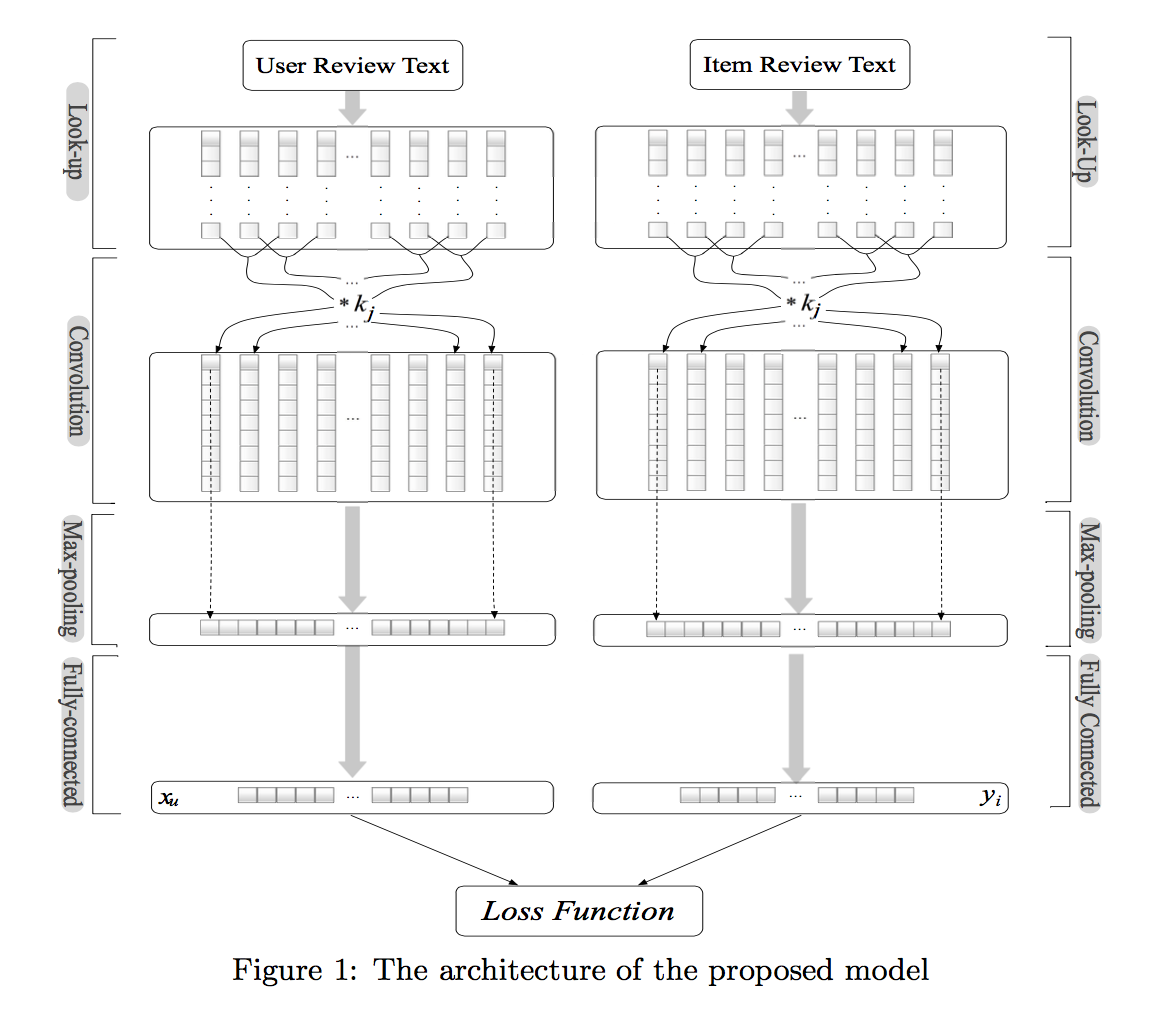
\includegraphics[scale=0.40]{DeepCoNN}
\caption{DeepCoNN Architecture}
\end{center}
\end{figure}

Note that in the original paper the first layer of the network is a "lookup" layer that transforms review text into embeddings. As discussed above, we create embedding prior to feeding into the network thus we omit a explicit "lookup" layer. Since the embedding layer uses pre-trained embedding and this is non-trainable our method is similar. The table on the following page summarizes our baseline DeepCoNN-DP model.  


\begin{figure}[!ht]
\begin{center}
{
\begin{tabular}{ |p{3cm}|p{1cm}| }
 \hline
 \multicolumn{2}{|c|}{\textbf{Baseline DeepCoNN-DP Model}} \\
 \hline
 \textbf{CNN Layer} & 1  \\
 $Hidden Size$ & 64 \\
 $Filters$   & 2    \\
 $Kernel Size$ &   8\\
 $Strides$ & 6 \\
 $Activation$    & ReLU \\
 \hline
 \textbf{Max Pooling} &   1  \\
   \hline
 \textbf{Flattened} & 1    \\
  \hline
 \textbf{Fully-Connected} & 1  \\
  $Hidden Size$ & 32 \\

 \hline
\end{tabular}
}
\end{center}
\caption{DeepCoNN Baseline Architecture}
\end{figure}


To train two networks simultaneously using a single loss function, the paper combines the outputs of both networks by concatenation. From here the interaction of user review features with movie review features is done via a \textit{factorization machine} (FM) of which the details are not provided. However, the goal of the FM is to capture second-oder interactions between users and movies. The $DeepCoNN$ loss function including FM:

$$
\textbf{DeepCoNN-FM} = \hat{\beta_{0}} + \sum_{i=1}^{\hat{|z|}}\hat{w_{i}}\hat{z_{i}} + \sum_{i=1}^{\hat{|z|}} 
\sum_{j=i+1}^{\hat{|z|}} \langle \hat{v_i}, \hat{v_j} \rangle \hat{z_i}\hat{z_j}
$$
\textbf{Where:}\\
$\hat{\beta_0}$ is the global bias\\
$\hat{w_i}$ models strength of $i^{th}$ variable in $\hat{z}$\\
$\langle\hat{v_i}, \hat{v_j} \rangle$ is the $2^{nd}$ order interaction\\


After contacting the authors, we were told that taking the dot product of the output from the fully connected layers of $Net_{u}$ and $Net_{i}$ should closely resemble the factorization machine approach and results focusing on first-order interactions. These results are further discussed in the conclusions and results section. The loss function for the dot product approach is defined as follows:

$$
\textbf{DeepCoNN-DP} = \hat{\beta_{0}} + \sum_{i=1}^{\hat{|z|}}\hat{w_{i}}\hat{z_{i}} + x^{T}_{u}x_{i}
$$

Optimization in the paper is done via $RMSprop$ which we replicated. However in further experiments we switched to $Adam$ after finding it led to similar results. Hence we decided to use $Adam$ in all experimental architectures to ensure consistency between models. $Adam$ is an adaptive version of gradient descent that controls the step size with respect to the absolute value of the gradient. Lastly, note that the paper did not mention of the use of regularization.

\begin{figure}[!ht]
\begin{center}
{\small
\begin{tabular}{l|cccccc}
\hline
%Category & Experiment Summary  \\ \hline
& \textbf{CNN} & \textbf{LSTM} & \textbf{GRU}  \\
\hline
\textbf{GloVe Embedding} & 50 $|$ 100 & 50 $|$ 100 & 50 $|$ 100 \\
\hline
\textbf{Hidden Layer} & 1 & 1 & 1 \\
$Units$ & 64 & 64 & 64 \\
$Activation$ & ReLU & Tanh &  Tanh \\
$Dropout$ \% & 0.10 & 0.10 & 0.10 & \\
\textit{Recurrent Drop.} \% & \-- & 0.20 & 0.20 & \\
\hline
\textbf{Dense Layer} & 1 & 1 & 1 \\
$Units$ & 64 & 64 &  64 \\
$Activation$ & ReLU & ReLU &  ReLU \\
\hline
\textbf{Optimizer} & Adam & Adam &  Adam \\
\hline

\end{tabular}
}
\end{center}
\caption{DeepCoNN Architecture Comparisons}
\end{figure}

\subsubsection{CNN Architecture}
CNNs are very popular within the image processing field and its applications.
For text applications, similar to image processing, CNNs make use of temporal convolution operators known as filters. In practice, filters are applied at multiple resolutions and coupled with non-linear activation functions
and pooling techniques such as max pooling. The convolution operation is a linear mapping over “n-gram vectors” which helps learn word representations. See Figure 1 for a depiction of the architecture used in the original paper.

In our initial model experiments we decided to innovate upon the $DeepCoNN$ model by adding regularization via dropout, and expand the number of neurons in the hidden (CNN) and dense layers. Additionally, for consistency when experimenting between models we utilized $Adam$ as our optimizer. Our implementation of this is detailed in Figure 2 above.

\subsubsection{LSTM Architecture}
Long Short-Term Memory (LSTM) cells retain and control information flow outside the normal flow of a simply recurrent network (RNN) via the use of gated cells. Symbolically, information can be stored, written, or read from a cell, similar to how data is manipulated in a computer’s memory. LSTM cells "decide" what is stored, written, or read by opening and closing gates. In practice these actions are implemented with element-wise multiplication by sigmoids which range from zero to one. A graphical overview of an LSTM cell is depicted below in Figure 3 [14]. A summary of our implementation can be found in Figure 2 above.

Thus gates can block or pass on information based on its strength, which they control through their own sets of weights. LSTMs are well-known variants of traditional RNNs and were introduced by Hochreiter and Schmidhuber in 1997 [16]. Furthermore, they are popular with the natural language processing given their above abilities, addition to, their ability to counteract the vanishing-gradient problem; and because standard stochastic gradient descent-based learning techniques can be used given their differentiability. The downside of LSTMs is the magnitude of parameterizations increases leading to longer training times, which we discuss in the results section. As discussed above, in all of our experiments we implemented regularization via recurrent dropout and/or regular dropout. We also expanded the number of hidden units and changed the optimizer.  

\begin{figure}[!ht]
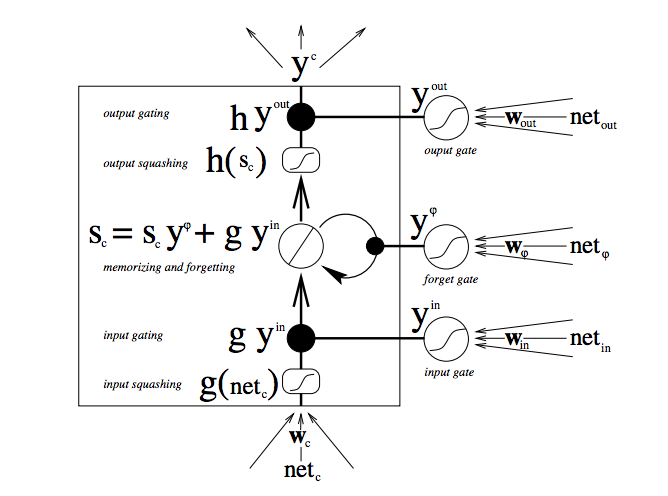
\includegraphics[scale=0.38]{LSTM.png}
\caption{LSTM Gated Cell}
\end{figure}

\subsubsection{GRU Architecture}
We also explored Gated Recurrent Units (GRU) which were introduced in 2014 by Cho et al. [15]. GRUs simplify the LSTM architecture by combing the forget and input gates into an update gate and merging the cell state with the
hidden state. Thus GRU have fewer gates than LSTMs and eliminate the separate memory component. As you would expect, this leads to fewer parameterizations. Figure 4 shows the mathematics of GRU gates [16]. A summary of our implementation can be found in Figure 2 above.

\begin{figure}[!ht]
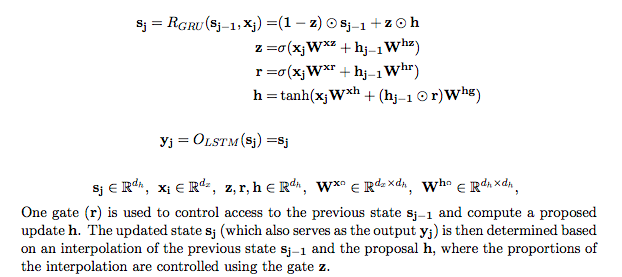
\includegraphics[scale=0.40]{GRU.png}
\caption{GRU Mathematical Overview}
\end{figure}

\subsection{Implementation Details}

To implement the DeepCoNN-DP model we used $Python$. Modeling construction was done via $Keras$ version 2.1.2 with a $TensorFlow$ version 1.4.0 back end. Data preprocessing was done mainly via $pandas$, $numpy$, \textit{Keras preprocessing API}, and $sklearn$. Please see the project \href{https://github.com/michaelAlvarino/Deep-Learning}{GitHub} repository for specific code implementation details. For training we used one Tesla K80 GPU on Google Cloud.

\subsection{Results}

Our preliminary work consisted of implementing DeepCoNN to model text review data for movie rating prediction. We then tried to innovate upon the DeepCoNN framework by experimenting with two new architectures in the $LSTM$ DeepCoNN-DP model and $GRU$ DeepCoNN-DP models as outlined above. Additionally, experimentation was done with the original CNN underlying architecture through regularization, hidden layer dimensionality, and optimizers. Equally important, we experimented with different GloVe word embeddings. Below we present and summarize those results.

We used our recreation of DeepCoNN-DP as the baseline model when comparing experiments. Mean squared error (MSE) was used when comparing models. Exhibit 1 shows our training/testing split as part of the data preprocessing step.
$$
\mbox{MSE} = \frac{1}{N}\sum_{n=1}^{N}(r_{n} - \hat{r}_{n})^2
$$

In the original paper the Amazon Music Instant Review data set was used. We have included a table in Figure 5 showing the original results of the authors from that experiment for convenience. Note that they achieved an MSE of 1.253 on the Amazon Music data set for the \textit{DeepCoNN-DP} model and a MSE of 1.233 on the \textit{DeepCoNN-FM} model. 

\begin{figure}[!ht]
\begin{center}
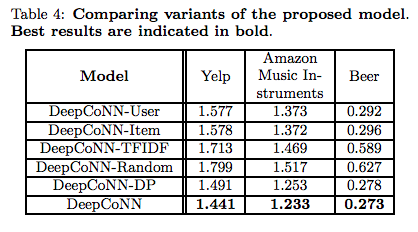
\includegraphics[scale=0.50]{orig_mses.png}
\caption{JDM MSE Results - Amazon Music Instruments}
\end{center}
\end{figure}

From our experiments using the Amazon Movie Review data set we show that all experiments lead to similar MSE results as per the paper's findings. Our results from all architectures use the dot product  (DeepCoNN-DP)  to capture user/movie interactions instead of the papers final model of (DeepCoNN-FM). After contacting the authors of the paper they recommended to use the dot product to capture interactions since the factorization machine method omitted specifications in the paper. Moreover despite considerable efforts, we were not ability to incorporate a factorization machine methodology from scratch.   

%\FloatBarrier
\begin{figure}[!h]
%\begin{exhibit}
\begin{center}
{\small
\begin{tabular}{l|cccc}
\hline
%Category & Experiment Summary  \\ \hline
 & Embedding & Avg pp. epoch (sec) & MSE Loss \\
\hline
DC-DP & 50d & 48.8 & 1.4505   \\
\textbf{GRU}& \textbf{50d}& \textbf{301.1}& \textbf{1.3683} \\
LSTM & 50d & 400.4 & 1.4775  \\

\hline
\end{tabular}
}
\end{center}
\caption{Results - 50d GloVe Model Comparisons}
\end{figure}

\begin{figure}[!h]
%\begin{exhibit}
\begin{center}
{\small
\begin{tabular}{l|cccc}
\hline
%Category & Experiment Summary  \\ \hline
 & Embedding & Training Time (sec) & MSE Loss \\
\hline
DC-DP & 100d  & 57.8 & 1.4635   \\
\textbf{GRU}& \textbf{100d}& \textbf{355.6}& \textbf{1.3901} \\
LSTM & 100d & 459.5 & 1.4888  \\

\hline
\end{tabular}
}
\end{center}
\caption{Results - 100d GloVe Model Comparisons}
\end{figure}

\subsubsection{Architecture Experiments}
Our first innovation beyond the described DeepCoNN model involved testing two new network architectures: an LSTM network and a GRU network. Of the two networks, the GRU model showed the most significant improvements in MSE vs our baseline DC-DP implementation. The LSTM model performed the worst. The GRU model had an MSE of 1.3683 using GloVe 50d embeddings and truncating user and movie reviews to the 40\% and 15\% respectively. Counter-intuitive to expectations, increasing the size of the GloVe embeddings did not improve the MSE of any model. This suggests that the vocab of the review corpus may differ from the GloVe corpus. We discuss solutions and tests for this further in the conclusions and future work sections. A summary of results per architecture and embedding is presented in Figure 6.

The downside of the RNN architectures particularly the LSTM was that training times were significantly slower than the baseline DeepCoNN-DP using a CNN architecture. In Figure 7 we can see that training the LSTM took \textbf{40\% longer} than training the GRU and almost \textbf{fourteen} times longer than the baseline model using one Tesla K80 GPU. Thus significant compute resources and time must be allocated to train these RNN networks relative to the CNN baseline. Consequently, this may limit their real-world application for companies with prohibitive resource or latency constraints. Lastly, we performed naive experimentation with different hyperparameters such as optimizer learning rates and dropout \%, but found that tuning only led to marginal differences and a more robust hyperparameter search was needed if given more time.

\subsubsection{Embedding Experiments}
As discussed above using GloVe embeddings has several advantages and disadvantages however we felt the advantages were greater. Intuitively, using pre-trained embeddings could help with the cold start problem that occurs in textual models when initially trying to learn a vocab from a new corpus. After implementing our new architectures we further innovated by testing the performance of different GloVe embeddings, namely 50d vs 100d. GloVe 100d increases the token size from roughly 400,000 unique tokens to roughly 1.5 million tokens. While increasing the vocab may help the model capture word representations from previously unknown words, the risk was that this was diminutive if the movie review corpus differs significantly from the movie review text corpus. 

Results show that the increased token size led to improved performance as noted in Figure 6. Particularly, on our best model (GRU DeepCoNN-DP) we saw a 0.07 decrease in MSE from 50d to 100d. Comparing across models we saw decreases in each architecture when increasing GloVe from 50d to 100d.\\

\subsubsection{Regularization}

We experimented with dropout regularization in all architectures, plus recurrent dropout in the RNN architectures. While the original paper did not use regularization in the baseline CNN architecture, LSTMs/GRUs have a tendency to easily over-fit and regularization is typically prudent. Below we show loss curves for all of our architectures using the 100d GloVe embeddings. For the LSTM and GRU architectures we used a recurrent dropout (removing layers) and standard dropout of masking the activation of some nodes. From the graphs we can see that even with regularization both the LSTM network and GRU network begin to over-fit half way through training. From our experiments we found that modest regularization helped smooth the loss curve and decrease over-fitting. For the CNN architecture, we found over-fitting to be less apparent which may be why the authors in the original paper omitted specifics on regularization. Regularization is summarized in Figure 2.


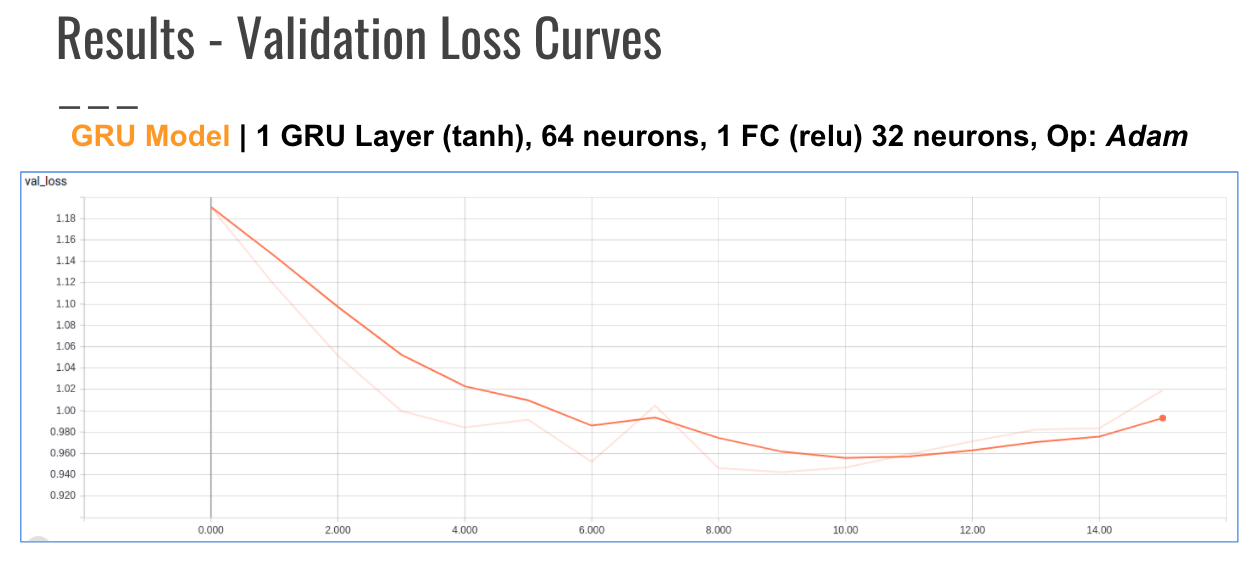
\includegraphics[scale=0.38]{Loss_Graph.png}

\section{Conclusion}

The textit{DeepCoNN} model represents a step forward in recommendation systems and the typical collaborative and content-based filtering systems that are traditionally used in recommendation systems. This was confirmed by the research contained in this research on predicting movie rankings. Our research indicates that the textit{DeepCoNN} model can be incrementally improved by utilizing different word embedding structures and regularization via dropout. Moreover, our research shows that significant improvement to prediction accuracy is available by implementing the textit{DeepCoNN} model with different architectures, namely the LSTm and GRU architectures described above. The tradeoff with LSTM and GRU architectures is that they are significantly more complex and also more time consuming to train. Practitioners may well continue to focus on collaborative filtering and the standard textit{DeepCoNN} model for these reasons, however with improved compute power the LSTM and GRO architectures would certainly overcome the training time disadavantage. 

We conclude that the \textit{DeepCoNN} model shows superior performance over standard collaborative filtering techniques and the Wide and Deep model proposed by Google researchers. Our research into other architectures and regularization methods confirm that further improvements to \textit{DeepCoNN} are available and further research into this model is certainly warranted. 






%Exhibit2
\begin{figure}[!ht]
\begin{center}
{\small
\begin{tabular}{l|ccccccc}
\hline
%Category & Experiment Summary  \\ \hline
Model & MSE & Training Time & Epochs \\
\hline
DeepCoNN-DP & 1.2645 & 10 min & 20  \\
\hline
\end{tabular}
}
\end{center}
\caption{DeepCoNN-DP Initial Results}
\end{figure}


\section{References}

[1] Zheng, Lei, Noroozi, Vahid and Yu, Philip. 
Joint Deep Modeling of Users and Items Using Reviews for Recommendations. arXiv working paper, June 2017

[2] Rendle, Steffan. 
Factorization Machines. ICDM 2010

[3] Catherine, Rose and Cohen, William. 
TransNets: Learning to Transform for Recommendation. arXiv working paper, June 2017

[4] Huifeng Guo, Ruiming Tang, Yunming Ye, Zhenguo Li, and Xiuqiang He
DeepFM: A Factorization-Machine based Neural Network for CTR Prediction
arXiv working paper, March 2017

[5] Heng-Tze Cheng, Levent Koc, Jeremiah Harmsen, Tal Shaked, Tushar Chandra, Hrishi Aradhye, Glen Anderson, Greg Corrado, Wei Chai, Mustafa Ispir, Rohan Anil, Zakaria Haque, Lichan Hong, Vihan Jain, Xiaobing Liu, and Hemal Shah.
Wide \& Deep Learning for Recommender Systems. arXiv working paper, June 2016

[6] A. Baylen. Github Repo $Uifud$
https://github.com/Praznat/uifud
As of 11/27/17 

[7] J.Pennington, R. Socher, C.Manning. 
Global Vectors for Word Representation version: 6B.50d.txt. 
https://nlp.stanford.edu/projects/glove/ 
Available as of 11/27/17 

[8] J. McAuley, C. Targett, J. Shi, A. van den Hengel Sigir, 2015
Image-based recommendations on styles and substitutes

[9] Balakrishnan Anusha, Dixit Kalpit. 
DeepPlaylist: Using Recurrent Neural Networks to Predict Song Similarity. semanticscholars.org 

[10] Young-Jun Ko, Lucas Maystre, Matthias Grossglauser, 2016
Collaborative Recurrent Neural Networks for Dynamic Recommender Systems
 
[11] David Zhan Liu, Gurbir Singh
A Recurrent Neural Network Based Recommendation System

[12] Bhuwan Dhingra, Hanxiao Liu, Ruslan Salakhutdinov, William W. Cohen
A Comparative Study of Word Embeddings for Reading Comprehension

[13] A Beginner's Guide to Recurrent Neural Networks and LSTMS
https://deeplearning4j.org/lstm.html

[14] Kyunghyun Cho, Bart van Merrienboer, C¸ aglar G¨ul¸cehre, Fethi Bougares, Holger Schwenk, and Yoshua Bengio., 2014 
Learning phrase representations using RNN encoder-decoder for statistical machine translation.

[15] Yoav Goldberg, draft 2015
A Primer on Neural Network Models for Natural Language Processing

[16] Hochreiter and Schmidhuber in 1997



\end{document}
